%=====================================================================
\section{Negative winding in ellipses: is the shape effect elastic or active?}\label{sec:smirror}
With positive winding the wall layer is made of self-propelled $+\half$, so its loss in elongated cavities could come from either of two
mechanisms: (1) \emph{lost shielding} (elastic and sign-symmetric: an evenly spaced layer cannot screen a non-circular interior,
Sec.~\ref{sec:theory}), or (2) \emph{motility and flow} (the two-vortex flow carries the motile wall $+\half$ off the wall). With negative winding
the wall carries $-\half$, which are not self-propelled. Mechanism (1) predicts a disrupted $-\half$ layer, more annihilation of bulk $+\half$ at the
wall and a smaller positive bulk in ellipses; mechanism (2) predicts that the $-\half$ layer survives elongation.

\paragraph{Runs.} \texttt{runs/cassini/P6\_mirror\_shapes/}: circle and ellipses $\varepsilon=1.2$, 1.5, 2.0 of area 2500 ($\sqrt{A/\pi}=1.27\,\la$,
arclength anchoring, eMode 2) at $k=-6$ ($\rho\approx0.06$--0.07) and $k=-12$ ($\rho\approx0.12$--0.14), 2 seeds, 10k + 100k steps, outputs as the
positive-winding ellipses; passive references (circle and $\varepsilon=2.0$ at $k=-6$, $-12$). \textbf{Validation:} the passive references carry
exactly $2|k|$ $-\half$ (12.00 and 23.99 per frame) and no $+\half$, the first check of eMode 2 with negative winding.
Analyses: \texttt{wall\_sign\_analysis.py} (sign-aware wall lattice, travel, survival, charge; \texttt{data/mirror\_shapes\_wall.tsv}) and
\texttt{shielding\_test.py} (\texttt{data/shielding\_mirror\_*.tsv}).

\begin{figure}[H]\centering
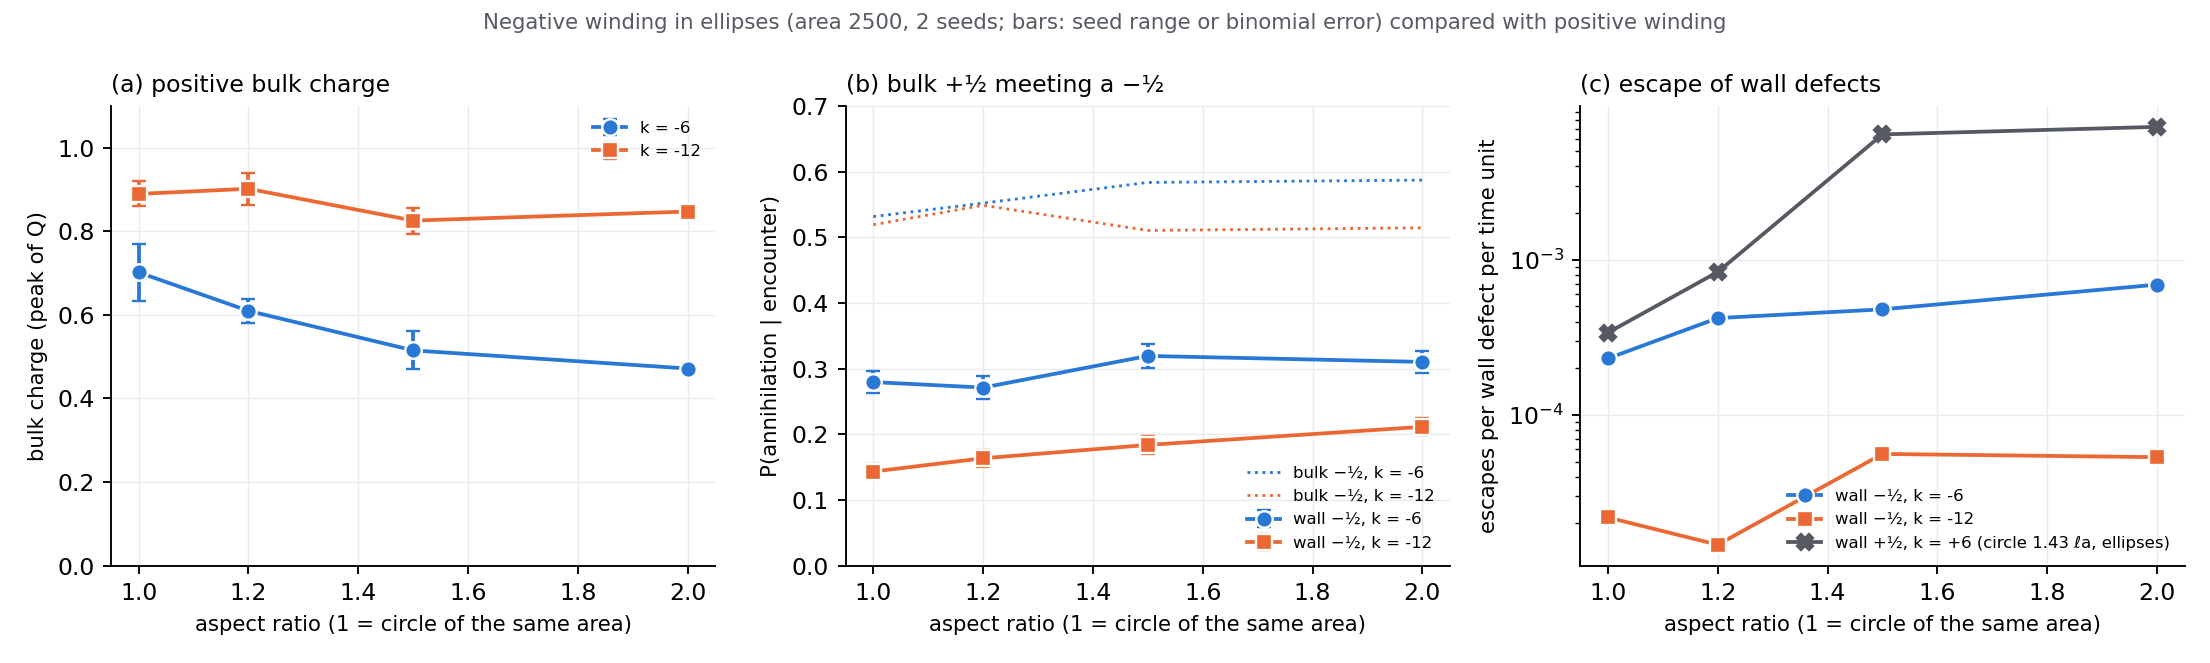
\includegraphics[width=\textwidth]{mirror_ellipses.png}
\caption{\textbf{Negative winding in ellipses.} (a) Positive bulk charge (peak of $Q$) against aspect ratio, $k=-6$ and $-12$. (b) Probability that an
encounter of a bulk $+\half$ with a $-\half$ ends in annihilation: wall targets (solid) and bulk targets (dotted). (c) Escape rate of wall defects:
$-\half$ (negative winding) and, for comparison, $+\half$ in positive-winding ellipses of the same area and the circle of $1.43\,\la$ (grey). 2 seeds;
bars: seed range in (a), binomial error in (b).}\label{fig:smirror}
\end{figure}
\begin{table}[H]\centering\small
\caption{Negative winding in ellipses (2 seeds; ranges over seeds). Occupancy: wall $-\half$ per frame over $2|k|+2$; pinning: static fraction of
the wall lattice at $m=2|k|+2$; escape: per wall defect per time unit; annihilation: probability that an encounter of a bulk $+\half$ with a wall
$-\half$ ends in annihilation (with a bulk $-\half$ in brackets).}\label{tab:smirror}
\begin{adjustbox}{max width=\textwidth}
\begin{tabular}{llcccc}\toprule
& & circle & $\varepsilon=1.2$ & $\varepsilon=1.5$ & $\varepsilon=2.0$\\\midrule
$k=-6$ & bulk charge & 0.63--0.77 & 0.58--0.64 & 0.47--0.56 & 0.46--0.48\\
& wall occupancy & 0.95--0.97 & 0.94--0.95 & 0.93--0.94 & 0.93\\
& pinning $f$ & 0.56--0.72 & 0.65--0.77 & 0.29--0.43 & 0.22--0.32\\
& escape ($10^{-4}$) & 2.3 & 4.1--4.3 & 4.8 & 6.4--7.4\\
& annihilation at the wall (bulk) & 0.28 (0.53) & 0.27 (0.55) & 0.32 (0.58) & 0.31 (0.59)\\\midrule
$k=-12$ & bulk charge & 0.86--0.92 & 0.86--0.94 & 0.79--0.86 & 0.84--0.86\\
& wall occupancy & 0.99 & 0.99 & 0.99 & 0.99\\
& pinning $f$ & 0.59--0.85 & 0.68--0.69 & 0.62--0.69 & 0.55--0.60\\
& escape ($10^{-4}$) & 0.2 & 0.1--0.2 & 0.5--0.6 & 0.5--0.6\\
& annihilation at the wall (bulk) & 0.14 (0.52) & 0.16 (0.55) & 0.18 (0.51) & 0.21 (0.51)\\\bottomrule
\end{tabular}
\end{adjustbox}
\end{table}
\begin{itemize}
  \item \textbf{The $-\half$ wall layer survives elongation.} Occupancy stays at 0.93--0.99 and the wall $-\half$ rarely leave: the escape rate rises
        $\approx3\times$ from the circle to $\varepsilon=2$, against $\approx20\times$ for the wall $+\half$ with positive winding (Fig.~\ref{fig:smirror}c).
        The layer loses its lattice order along the wall at $k=-6$ (pinning 0.56--0.77 $\to$ 0.22--0.32), but its defects stay at the wall.
  \item \textbf{Shielding weakens a little, as the elastic theory predicts.} A bulk $+\half$ meeting a wall $-\half$ annihilates somewhat more often in
        elongated cavities (0.28 $\to$ 0.31 at $k=-6$, 0.14 $\to$ 0.21 at $k=-12$), still far less often than with a bulk $-\half$ (0.51--0.59). At $k=-6$
        the positive bulk shrinks from $\approx0.7$ to $\approx0.47$; at $k=-12$ (crowded wall) there is no shape effect.
  \item \textbf{Conclusion.} Both mechanisms act, with very different strengths. Geometry weakens the elastic shielding for both signs, modestly
        (Sec.~\ref{sec:theory}); the dramatic loss of the layer with positive winding needs self-propelled wall defects, which the two-vortex flow carries
        off the wall. The shape effect of Part~III is therefore mainly an active effect enabled by geometry.
  \item The wall $-\half$ also travel along the wall in the circle (median 11--12 cells in 500 time units, 65\% beyond half a site spacing at $k=-6$),
        unlike wall $+\half$ in circles: the mirror wall layer creeps even without elongation, consistent with its lower pinning in the circle sweep
        (Sec.~\ref{sec:clattice}).
\end{itemize}
\open{Two seeds and one size; ovals with negative winding and a third seed would make this a main-text result (the office machine is free).}
